\subsection{A noisy physical-reflection sequence}
\label{sec:fresnel}
We generate a rocking air--dielectric interface from the Fresnel coefficients, with refractive index $1.5$ and incidence angle $\arctan(1.5)+18^{\circ}\cos(2\pi t/40)$ for $t=0,\ldots,40$. Unpolarized incident light gives normalized specular intensity one at Brewster's angle. Two polarization-orientation trajectories, three constant unpolarized background levels, two photon scales, and two seeds give 24 sequences and 984 frames per arm. Four ideal analyzer observations have independent Poisson shot noise and Gaussian read noise of standard deviation two electrons. We fit these observations with unweighted least squares.

Every solver/arm starts from $(0,0.2,-0.1)$ and inherits its own preceding raw endpoint. We use the existing $10^{-6}$ gradient tolerance, gap threshold, and local curvature gate, with at most one restart per frame. BFGS and L-BFGS-B report nine and seven inaccurate successes. Both curvature-triggered and physically audited branches have zero such endpoints, with seven interventions per solver; their corrections propagate through subsequent frames. On the uncorrected branches, the curvature gate detects all 16 false successes and flags no accurate accepted endpoint. The physical bound also rejects all 16. Both solvers have zero native failures in this grid. The simulation exhibits the fold mechanism under a specified physical noise model; direct physical auditing detects the same inaccurate endpoints. Supplementary Section S18 gives the complete protocol and alternative-map control.

\begin{figure*}[!t]
\centering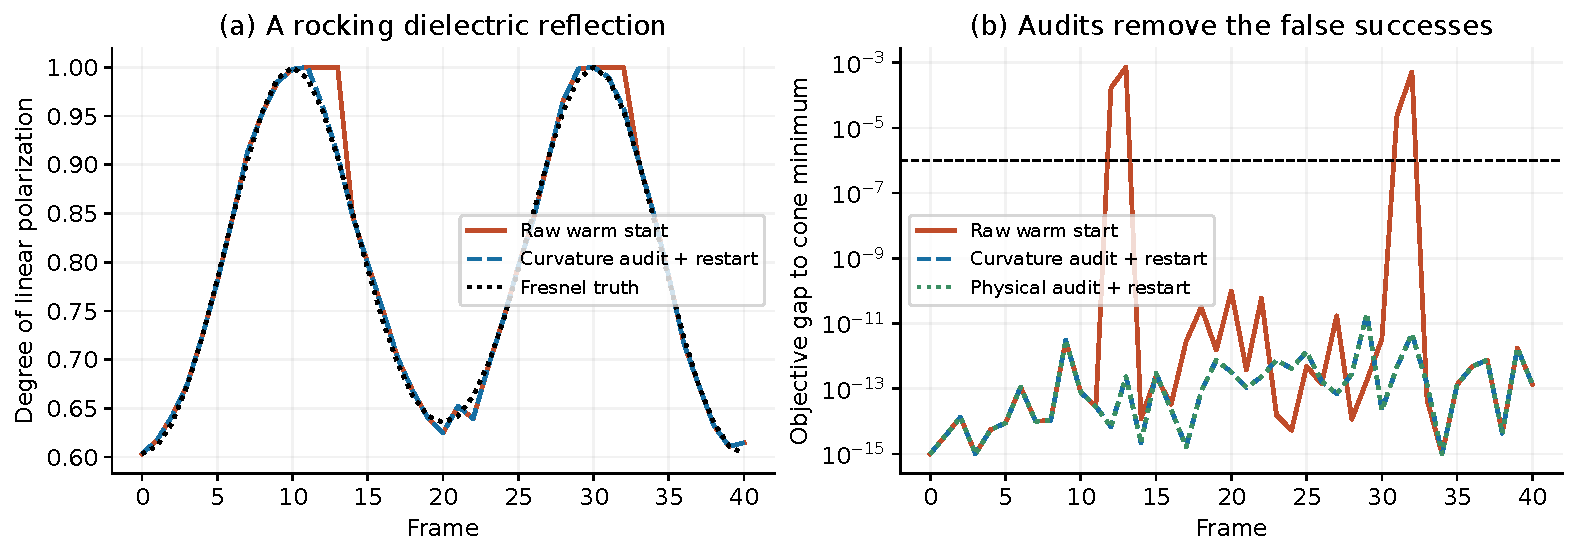
\includegraphics[width=.96\textwidth]{images/fresnel_sequence.pdf}
\caption{Fresnel-reflection continuation with shot and read noise. The displayed BFGS sequence is selected by the largest baseline objective gap in the fixed complete grid, rather than as a typical sequence. (a) Polarization estimate and physical truth. (b) Gap to the direct cone optimum; the dashed line is $10^{-6}$. Both audited branches overlap to plotting accuracy. Gaps below $10^{-15}$ are displayed at that floor. The complete grid has 984 frames per arm, with nine BFGS and seven L-BFGS-B false successes, versus zero in either audited branch.}
\label{fig:fresnel}
\end{figure*}

\subsection{Released polarization observations}
\label{sec:real}
We freeze small subsets of DeepSfP \cite{ba} and PolarNS/PolarBurstSR \cite{polarns} before optimization. DeepSfP contributes three indoor test objects and their four-angle observations. PolarNS contributes the lexicographically first object and scene mean/variance records, averaged over 10\,000 and 1\,017 captures. Those means are not treated as individual noisy frames. The first three released PolarBurstSR test crops contribute all 14 raw frames and four nominal color planes, unpacked with the authors' sensor layout.

For each static image, we select 128 seeded uniform eligible pixels and 64 pixels from an observed-high-DoLP stratum. For each burst color plane, a fixed $4\times4$ sensor grid is supplemented by eight high-DoLP positions selected using only the first frame. Finite, nonsaturated observations above a fixed relative intensity floor are eligible. The selections are reported separately in Supplementary Section S18; overlapping inputs and within-image/frame dependencies preclude a prevalence interpretation. Static samples follow a prescribed spatial scan. Burst samples follow fixed sensor coordinates without motion compensation, and are not asserted to follow one material point.

The reference is the cone optimum of the nominal four-analyzer quadratic. It measures optimization accuracy under that model; the available observations do not provide noise-free Stokes truth or a calibrated camera likelihood. Both solvers use $10^{-6}$ tolerance. Each arm carries its own state; a cold-start control resets intensity from the current observation and uses fixed polarization raw coordinates. The fixed protocol yields 576 DeepSfP, 384 PolarNS-mean, and 3\,682 burst entries per solver/arm, totaling 37\,136 fits across two solvers and four arms.

\begin{table*}[!t]
\caption{Released-data stopping audit. Every count pair is BFGS/L-BFGS-B. A false success is native acceptance with nominal quadratic gap above $10^{-6}$. Counts combine the separately reported sampling strata, not independent scenes. ``Detected'' and ``rejected'' refer to audits of the uncorrected warm-start endpoints. All native failure counts are zero.}
\label{tab:realdata}
\centering\small\renewcommand{\arraystretch}{1.15}
\begin{tabularx}{\textwidth}{@{}Xrrrrr@{}}\toprule
Subset & Entries & Cold false & Warm false & Local detected & Physical rejected\\\midrule
DeepSfP & 576 & 0/0 & 0/0 & 0/0 & 0/0\\
PolarNS means & 384 & 0/7 & 111/64 & 0/0 & 111/64\\
PolarBurstSR & 3\,682 & 0/7 & 16/104 & 0/0 & 16/104\\\bottomrule
\end{tabularx}
\end{table*}

Table~\ref{tab:realdata} shows inaccurate native successes in the PolarNS and burst subsets, while DeepSfP has none. None of the 295 uncorrected warm-start false successes satisfies the predeclared local fold gate, so curvature-triggered restarting leaves those counts unchanged. The physical bound rejects every inaccurate accepted endpoint. One physically audited radial restart leaves 68/64 native false successes in the PolarNS means and 16/99 in the bursts; their final bounds still reject them. The audit thus detects errors that a single radial restart leaves unresolved. On these observations, the physical stopping bound has broader coverage than the local fold gate. Figure~\ref{fig:realregimes} places them in the radius and gap-bound regimes.

An independent physical-coordinate SLSQP check of 29 selected reference minima has maximum loss discrepancy $1.31\times10^{-18}$. Independent float64 PyTorch AD audits all 309 cold/warm false successes and 32 control endpoints; maximum head-gradient, Hessian, and physical-gradient discrepancies are $7.77\times10^{-18}$, $8.89\times10^{-16}$, and $1.39\times10^{-17}$. No solver warning or native failure is removed. These checks assess the nominal objective and its derivatives. Aligned denoising, super-resolution, and surface-normal accuracy require separate evaluation.

\begin{figure*}[!t]
\centering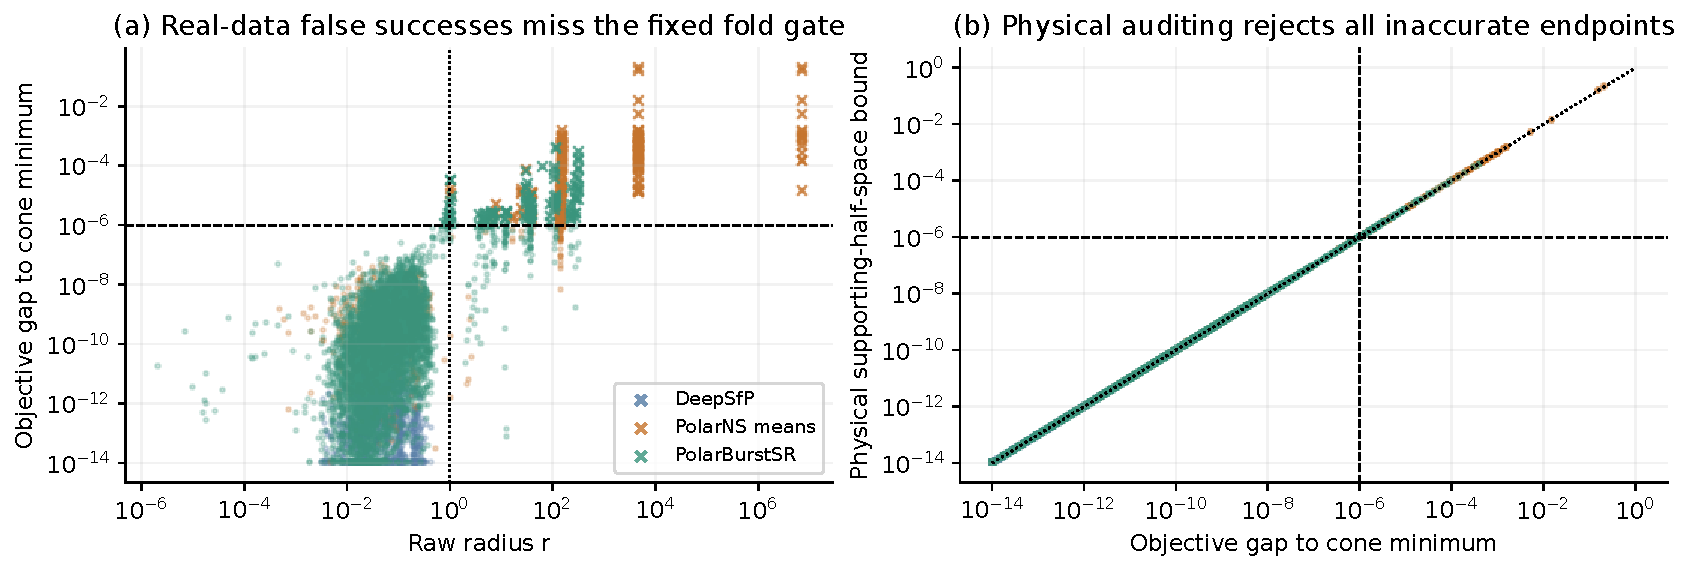
\includegraphics[width=.96\textwidth]{images/real_stopping_regimes.pdf}
\caption{All 9\,284 uncorrected real-data warm-start fits across two solvers. The subsets include uniform and enriched selections with repeated observations across distinct histories. (a) Objective gaps against raw radius. Crosses mark native false successes; the dotted line marks $r=1$ and the dashed line marks gap $10^{-6}$. None passes the fixed local fold gate. (b) Physical supporting-half-space bound against the reference gap; the dotted line is equality and dashed lines mark $10^{-6}$. The bound rejects all inaccurate endpoints. Values below $10^{-14}$ are displayed at that floor. The comparisons use float64 arithmetic, without outward-rounded certification.}
\label{fig:realregimes}
\end{figure*}

\subsection{Coordinate repair with physical stopping controls}
\label{sec:chartrepair}
The real-data failures motivate a follow-up on the same observations. We develop the repair rule after inspecting the previous audit, then freeze it before evaluation. The inputs, ordering, and thresholds are retained. Every arm carries its own preceding endpoint. Repeating the raw warm and cold branches reproduces all 18\,568 stored real-data endpoints exactly in raw coordinates.

For $r>1$, replacing $w$ by $C(w)=w/\|w\|^2$ preserves $F(w)$ and moves to the inner sheet. At fixed intensity and data, $\|\nabla_w\widetilde f(C(w))\|_2=r^2\|\nabla_w\widetilde f(w)\|_2$; the Jacobian condition number is unchanged. This relation follows from the paired preimages in Supplementary Section S6. A fresh solver invocation resets quasi-Newton memory. The fold and the dependence on intensity remain.

We compare applying this switch before every warm-start solve with a physically audited repair. On a bound rejection, the latter uses the existing radial trial rule if the local negative-curvature gate holds; otherwise it switches an outer endpoint and restarts once. Inner nonfold failures remain rejected. A control restarts once from the cold initialization instead. A guarded variant follows the coordinate repair with standard projected-gradient steps in physical coordinates when the bound still rejects. This fallback uses step one, at most 64 updates, and the same $10^{-6}$ bound threshold. No reference optimum initializes any iterative arm. A standalone physical projected-gradient solver and the direct cone solution are additional controls. Supplementary Section S19 specifies the algorithm and accounting.

\begin{table*}[!t]
\caption{Frozen coordinate-repair follow-up. Inaccurate means nominal gap above $10^{-6}$, irrespective of native or monitored acceptance. Count pairs are BFGS/L-BFGS-B, each with 4\,642 released-data entries and 984 Fresnel frames. Audited arms reject any remaining inaccurate outputs. Physical controls are single algorithms, without a head-solver pair. FG counts exclude separately recorded physical audits and Hessians.}
\label{tab:chartrepair}
\centering\small\renewcommand{\arraystretch}{1.12}
\begin{tabularx}{\textwidth}{@{}Xrrr@{}}\toprule
Strategy & Released inaccurate & Fresnel inaccurate & Released native FG pairs\\\midrule
Raw warm start & 127/168 & 9/7 & 92\,025/32\,235\\
Cold start & 0/14 & 0/0 & 97\,801/29\,468\\
Switch before each warm solve & 9/16 & 12/10 & 94\,974/32\,527\\
Audited cold restart & 0/2 & 0/0 & 95\,791/33\,232\\
Audited coordinate repair & 7/22 & 0/0 & 95\,640/33\,440\\
Coordinate repair with physical fallback & 0/0 & 0/0 & 95\,635/33\,245\\
Physical projected gradient & 0 & 0 & ---\\
Direct cone solution & 0 & 0 & ---\\\bottomrule
\end{tabularx}
\end{table*}

Table~\ref{tab:chartrepair} separates partial coordinate improvement from completed correction. Switching before each solve reduces released-data inaccurate endpoints from 295 to 25, but increases the Fresnel count from 16 to 22. The audited coordinate arm leaves 29 inaccurate released-data endpoints, all rejected. Adding physical fallback leaves none: BFGS and L-BFGS-B require respectively two and 15 fallback calls, with three and 22 projected updates in total. There are 4\,663/4\,704 physical-gradient queries in those guarded branches, including stopping audits. No real-data repair invokes the local curvature gate. In the Fresnel grid, each guarded solver uses seven full head-Hessian queries and 21 trial FG evaluations; neither requires physical fallback.

A separate paired-endpoint audit applies the repair to the same 9\,284 historical warm endpoints, rather than changed continuation histories. Coordinate repair leaves 7/39 of the original 127/168 inaccurate endpoints; physical fallback removes those remaining 46. Audited cold restarting leaves 0/5. Thus the coordinate-only step corrects 249 of the 295 original failures, while full correction depends on the physical fallback. Independent PyTorch checks cover all 295 historical false successes and 32 controls; the largest output-preservation and gradient-transformation discrepancies are $1.74\times10^{-18}$ and $7.78\times10^{-16}$.

The physical controls are substantially cheaper in this implementation. Across 4\,642 released entries, standalone projected gradient uses 9\,575 updates and 14\,217 physical-gradient queries, with no inaccurate or rejected outputs. Its observed time is 0.203 s, versus 4.64/1.35 s for the guarded head solvers and 0.0219 s for the direct cone solution. These timings describe one CPU pass in the stated implementation. Coordinate repair provides a partial remedy for existing head-based fits; the direct physical methods are more economical for this quadratic. All released-data repairs in this follow-up use first derivatives.

